\documentclass{standalone}
\usepackage{tikz}
\usetikzlibrary{patterns, positioning}
\usepackage[sfdefault]{ClearSans} %% option 'sfdefault' activates Clear Sans as the default text font
\usepackage[T1]{fontenc}

\begin{document}
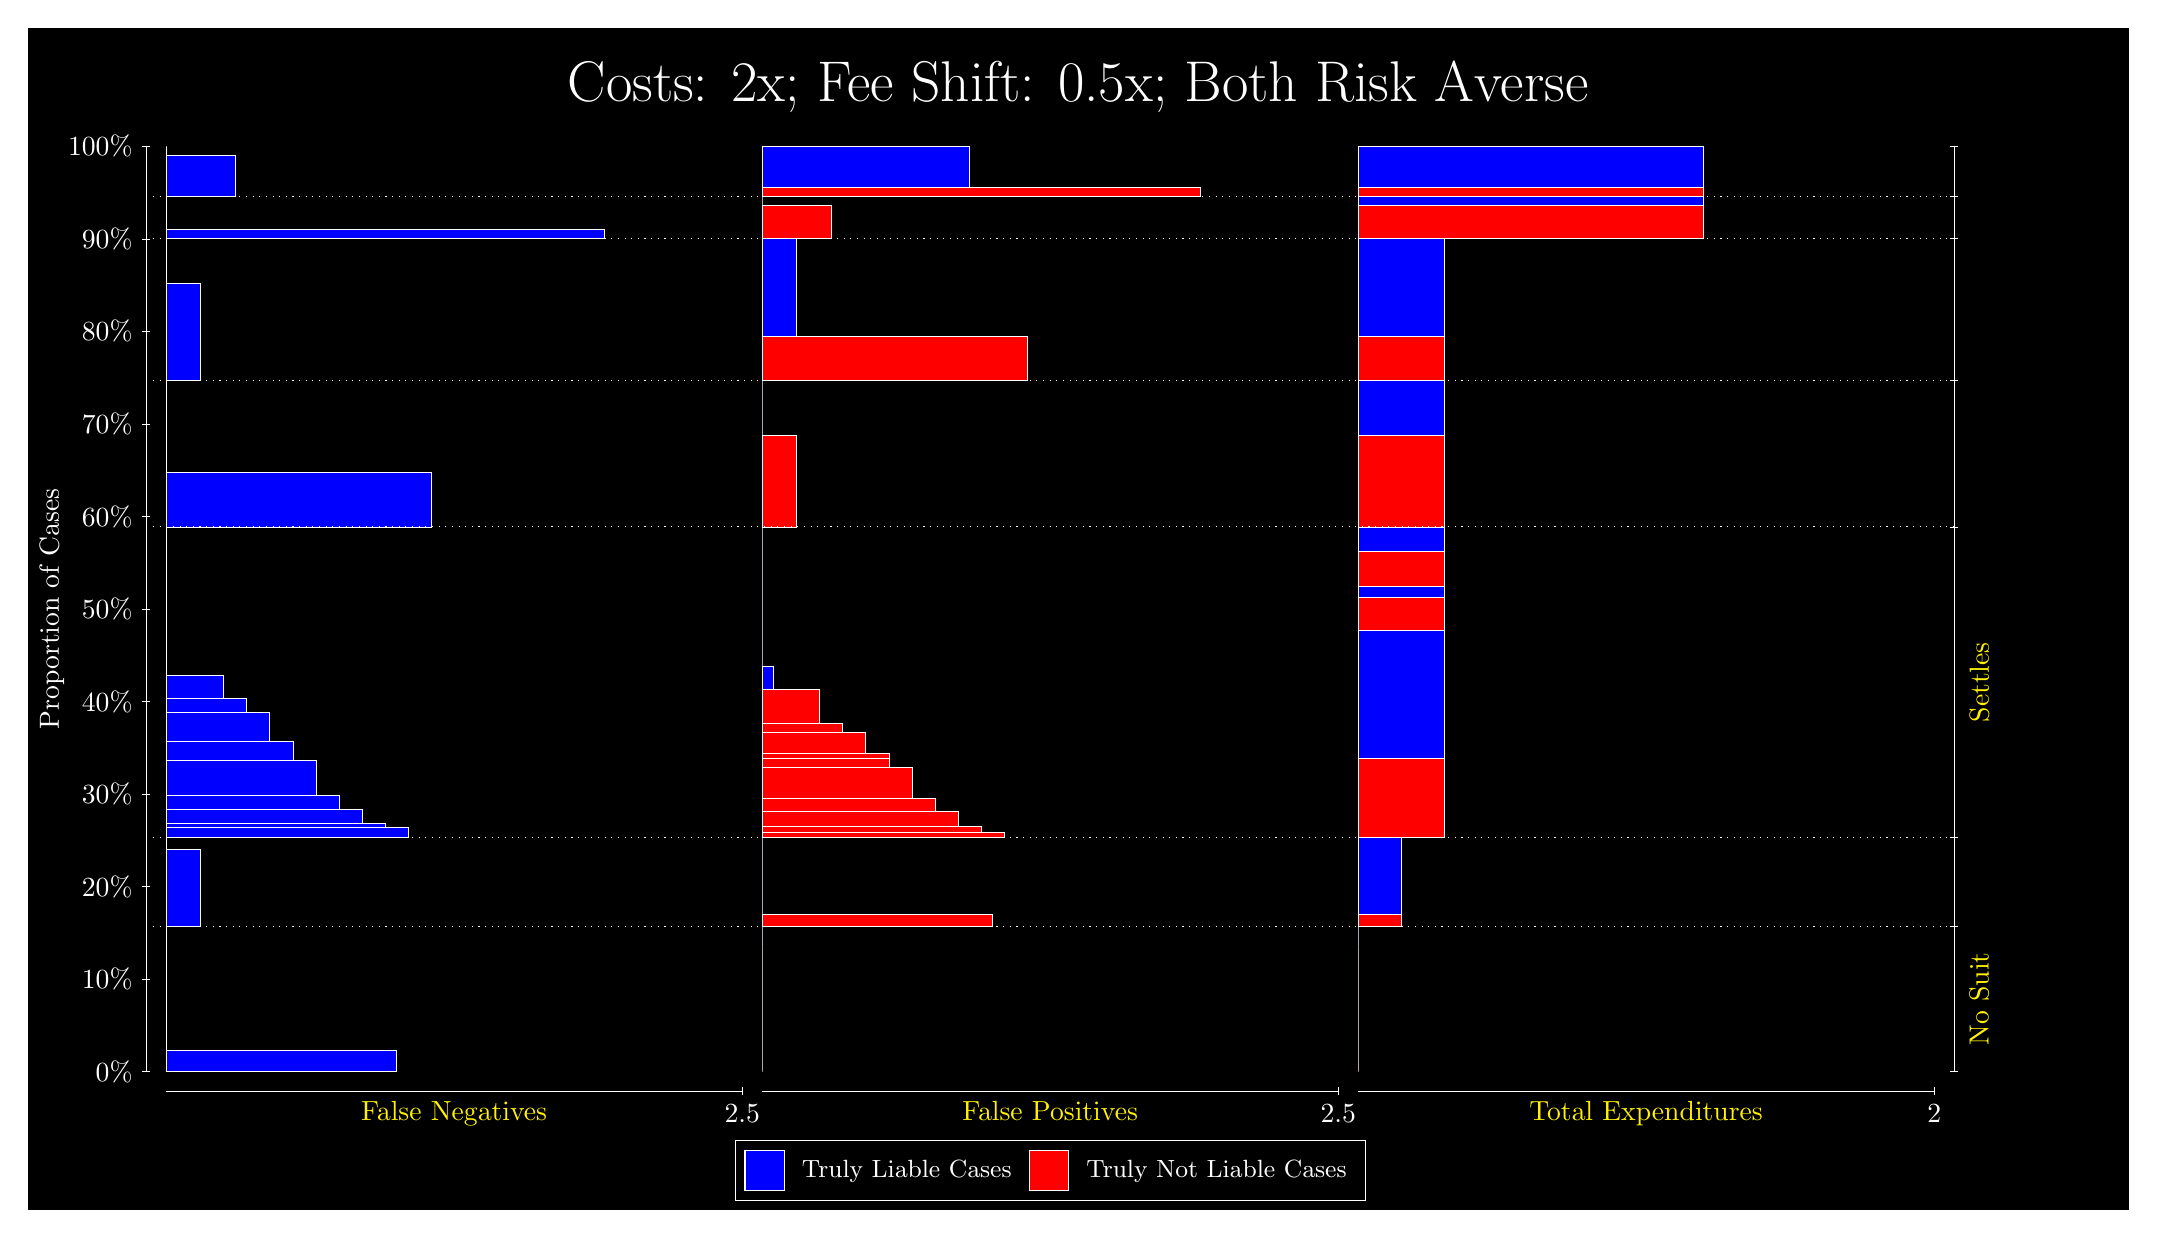
\begin{tikzpicture}
\draw[fill=black] (0,0) rectangle (26.667,15);
\draw[text=white] (0,13.5) rectangle (26.667,15) node[midway] {\huge Costs: 2x; Fee Shift: 0.5x; Both Risk Averse};
\draw[white, very thin] (1.5,1.75) -- (1.5,13.5);
\node[rotate=90, text=white, anchor=center] at (0.3, 7.625) {Proportion of Cases};
\draw[white, very thin] (1.45,1.75) -- (1.55,1.75);
\node[text=white, anchor=east] at (1.45, 1.75) {0\%};
\draw[white, very thin] (1.45,2.925) -- (1.55,2.925);
\node[text=white, anchor=east] at (1.45, 2.925) {10\%};
\draw[white, very thin] (1.45,4.1) -- (1.55,4.1);
\node[text=white, anchor=east] at (1.45, 4.1) {20\%};
\draw[white, very thin] (1.45,5.275) -- (1.55,5.275);
\node[text=white, anchor=east] at (1.45, 5.275) {30\%};
\draw[white, very thin] (1.45,6.45) -- (1.55,6.45);
\node[text=white, anchor=east] at (1.45, 6.45) {40\%};
\draw[white, very thin] (1.45,7.625) -- (1.55,7.625);
\node[text=white, anchor=east] at (1.45, 7.625) {50\%};
\draw[white, very thin] (1.45,8.8) -- (1.55,8.8);
\node[text=white, anchor=east] at (1.45, 8.8) {60\%};
\draw[white, very thin] (1.45,9.975) -- (1.55,9.975);
\node[text=white, anchor=east] at (1.45, 9.975) {70\%};
\draw[white, very thin] (1.45,11.15) -- (1.55,11.15);
\node[text=white, anchor=east] at (1.45, 11.15) {80\%};
\draw[white, very thin] (1.45,12.325) -- (1.55,12.325);
\node[text=white, anchor=east] at (1.45, 12.325) {90\%};
\draw[white, very thin] (1.45,13.5) -- (1.55,13.5);
\node[text=white, anchor=east] at (1.45, 13.5) {100\%};

\draw[white, very thin] (24.457,1.75) -- (24.457,13.5);
\draw[white, very thin] (24.407,1.75) -- (24.507,1.75);
\node[anchor=west] at (24.407, 1.75) {};
\draw[white, very thin] (24.407,3.5925) -- (24.507,3.5925);
\node[anchor=west] at (24.407, 3.5925) {};
\draw[white, very thin] (24.407,4.72) -- (24.507,4.72);
\node[anchor=west] at (24.407, 4.72) {};
\draw[white, very thin] (24.407,8.6666) -- (24.507,8.6666);
\node[anchor=west] at (24.407, 8.6666) {};
\draw[white, very thin] (24.407,10.525) -- (24.507,10.525);
\node[anchor=west] at (24.407, 10.525) {};
\draw[white, very thin] (24.407,12.326) -- (24.507,12.326);
\node[anchor=west] at (24.407, 12.326) {};
\draw[white, very thin] (24.407,12.864) -- (24.507,12.864);
\node[anchor=west] at (24.407, 12.864) {};
\draw[white, very thin] (24.407,13.5) -- (24.507,13.5);
\node[anchor=west] at (24.407, 13.5) {};

\draw[white, very thin, fill=blue] (1.75,1.75) rectangle (4.6775,2.0192);
\draw[white, very thin, fill=red] (1.75,2.0192) rectangle (1.75,3.5925);
\draw[white, very thin, fill=blue] (1.75,3.5925) rectangle (2.1891,4.5689);
\draw[white, very thin, fill=red] (1.75,4.5689) rectangle (1.75,4.72);
\draw[white, very thin, fill=blue] (1.75,4.72) rectangle (4.8239,4.8479);
\draw[white, very thin, fill=blue] (1.75,4.8479) rectangle (4.5312,4.9024);
\draw[white, very thin, fill=blue] (1.75,4.9024) rectangle (4.2384,5.0802);
\draw[white, very thin, fill=blue] (1.75,5.0802) rectangle (3.9457,5.2562);
\draw[white, very thin, fill=blue] (1.75,5.2562) rectangle (3.6529,5.7085);
\draw[white, very thin, fill=blue] (1.75,5.7085) rectangle (3.3602,5.9427);
\draw[white, very thin, fill=blue] (1.75,5.9427) rectangle (3.0674,6.3066);
\draw[white, very thin, fill=blue] (1.75,6.3066) rectangle (2.7746,6.4859);
\draw[white, very thin, fill=blue] (1.75,6.4859) rectangle (2.4819,6.7818);
\draw[white, very thin, fill=red] (1.75,6.7818) rectangle (1.75,8.6666);
\draw[white, very thin, fill=blue] (1.75,8.6666) rectangle (5.1167,9.3597);
\draw[white, very thin, fill=red] (1.75,9.3597) rectangle (1.75,10.525);
\draw[white, very thin, fill=blue] (1.75,10.525) rectangle (2.1891,11.763);
\draw[white, very thin, fill=red] (1.75,11.763) rectangle (1.75,12.326);
\draw[white, very thin, fill=blue] (1.75,12.326) rectangle (7.3123,12.442);
\draw[white, very thin, fill=red] (1.75,12.442) rectangle (1.75,12.864);
\draw[white, very thin, fill=blue] (1.75,12.864) rectangle (2.6283,13.384);
\draw[white, very thin, fill=red] (1.75,13.384) rectangle (1.75,13.5);
\draw[white, very thin, fill=red] (9.3189,1.75) rectangle (9.3189,3.3233);
\draw[white, very thin, fill=blue] (9.3189,3.3233) rectangle (9.3189,3.5925);
\draw[white, very thin, fill=red] (9.3189,3.5925) rectangle (12.246,3.7436);
\draw[white, very thin, fill=blue] (9.3189,3.7436) rectangle (9.3189,4.72);
\draw[white, very thin, fill=red] (9.3189,4.72) rectangle (12.393,4.7908);
\draw[white, very thin, fill=red] (9.3189,4.7908) rectangle (12.1,4.8655);
\draw[white, very thin, fill=red] (9.3189,4.8655) rectangle (11.807,5.0552);
\draw[white, very thin, fill=red] (9.3189,5.0552) rectangle (11.515,5.2189);
\draw[white, very thin, fill=red] (9.3189,5.2189) rectangle (11.222,5.6085);
\draw[white, very thin, fill=red] (9.3189,5.6085) rectangle (10.929,5.7246);
\draw[white, very thin, fill=red] (9.3189,5.7246) rectangle (10.929,5.7969);
\draw[white, very thin, fill=red] (9.3189,5.7969) rectangle (10.636,6.0553);
\draw[white, very thin, fill=red] (9.3189,6.0553) rectangle (10.344,6.1787);
\draw[white, very thin, fill=red] (9.3189,6.1787) rectangle (10.051,6.6049);
\draw[white, very thin, fill=blue] (9.3189,6.6049) rectangle (9.4652,6.9007);
\draw[white, very thin, fill=blue] (9.3189,6.9007) rectangle (9.3189,8.6666);
\draw[white, very thin, fill=red] (9.3189,8.6666) rectangle (9.758,9.8315);
\draw[white, very thin, fill=blue] (9.3189,9.8315) rectangle (9.3189,10.525);
\draw[white, very thin, fill=red] (9.3189,10.525) rectangle (12.686,11.087);
\draw[white, very thin, fill=blue] (9.3189,11.087) rectangle (9.758,12.326);
\draw[white, very thin, fill=red] (9.3189,12.326) rectangle (10.197,12.748);
\draw[white, very thin, fill=blue] (9.3189,12.748) rectangle (9.3189,12.864);
\draw[white, very thin, fill=red] (9.3189,12.864) rectangle (14.881,12.98);
\draw[white, very thin, fill=blue] (9.3189,12.98) rectangle (11.954,13.5);
\draw[white, very thin, fill=red] (16.888,1.75) rectangle (16.888,3.3233);
\draw[white, very thin, fill=blue] (16.888,3.3233) rectangle (16.888,3.5925);
\draw[white, very thin, fill=red] (16.888,3.5925) rectangle (17.437,3.7436);
\draw[white, very thin, fill=blue] (16.888,3.7436) rectangle (17.437,4.72);
\draw[white, very thin, fill=red] (16.888,4.72) rectangle (17.986,5.7246);
\draw[white, very thin, fill=blue] (16.888,5.7246) rectangle (17.986,7.3531);
\draw[white, very thin, fill=red] (16.888,7.3531) rectangle (17.986,7.7793);
\draw[white, very thin, fill=blue] (16.888,7.7793) rectangle (17.986,7.9072);
\draw[white, very thin, fill=red] (16.888,7.9072) rectangle (17.986,8.3613);
\draw[white, very thin, fill=blue] (16.888,8.3613) rectangle (17.986,8.6666);
\draw[white, very thin, fill=red] (16.888,8.6666) rectangle (17.986,9.8315);
\draw[white, very thin, fill=blue] (16.888,9.8315) rectangle (17.986,10.525);
\draw[white, very thin, fill=red] (16.888,10.525) rectangle (17.986,11.087);
\draw[white, very thin, fill=blue] (16.888,11.087) rectangle (17.986,12.326);
\draw[white, very thin, fill=red] (16.888,12.326) rectangle (21.279,12.748);
\draw[white, very thin, fill=blue] (16.888,12.748) rectangle (21.279,12.864);
\draw[white, very thin, fill=red] (16.888,12.864) rectangle (21.279,12.98);
\draw[white, very thin, fill=blue] (16.888,12.98) rectangle (21.279,13.5);
\draw[white, dotted] (1.5,3.5925) -- (24.457,3.5925);
\draw[white, dotted] (1.5,4.72) -- (24.457,4.72);
\draw[white, dotted] (1.5,8.6666) -- (24.457,8.6666);
\draw[white, dotted] (1.5,10.525) -- (24.457,10.525);
\draw[white, dotted] (1.5,12.326) -- (24.457,12.326);
\draw[white, dotted] (1.5,12.864) -- (24.457,12.864);
\draw[white, very thin] (1.75,1.5) -- (9.0689,1.5);
\node[text=yellow, anchor=north] at (5.4094, 1.5) {False Negatives};
\draw[white, very thin] (9.0689,1.45) -- (9.0689,1.55);
\node[text=white, anchor=north] at (9.0689, 1.45) {2.5};

\draw[white, very thin] (9.3189,1.5) -- (16.638,1.5);
\node[text=yellow, anchor=north] at (12.978, 1.5) {False Positives};
\draw[white, very thin] (16.638,1.45) -- (16.638,1.55);
\node[text=white, anchor=north] at (16.638, 1.45) {2.5};

\draw[white, very thin] (16.888,1.5) -- (24.207,1.5);
\node[text=yellow, anchor=north] at (20.547, 1.5) {Total Expenditures};
\draw[white, very thin] (24.207,1.45) -- (24.207,1.55);
\node[text=white, anchor=north] at (24.207, 1.45) {2};

\node[text=yellow, centered, rotate=90] at (24.777, 2.6712) {No Suit};

\node[text=yellow, centered, rotate=90] at (24.777, 6.6933) {Settles};





\draw (12.978300999999998,1.5) node[draw=none] (baseCoordinate) {};
\begin{scope}[align=center]
        \matrix[scale=0.5, draw=white, below=0.5cm of baseCoordinate, nodes={draw}, column sep=0.1cm]{
            \node[rectangle, draw, minimum width=0.5cm, minimum height=0.5cm, fill=blue] {}; &
            \node[draw=none, font=\small, text=white] (B) {Truly Liable Cases}; &
            \node[rectangle, draw, minimum width=0.5cm, minimum height=0.5cm, fill=red] {}; &
            \node[draw=none, font=\small, text=white] (B) {Truly Not Liable Cases}; \\
            };
\end{scope}

\end{tikzpicture}
\end{document}